\documentclass[border=10pt]{standalone}

\usepackage{tikz}
\usepackage{tikzsymbols}
\usetikzlibrary{calc,patterns,shapes.geometric}

\def\centerarc[#1](#2)(#3:#4:#5){\draw[#1] ($(#2)+({#5*cos(#3)},{#5*sin(#3)})$) arc (#3:#4:#5);}

\begin{document}
	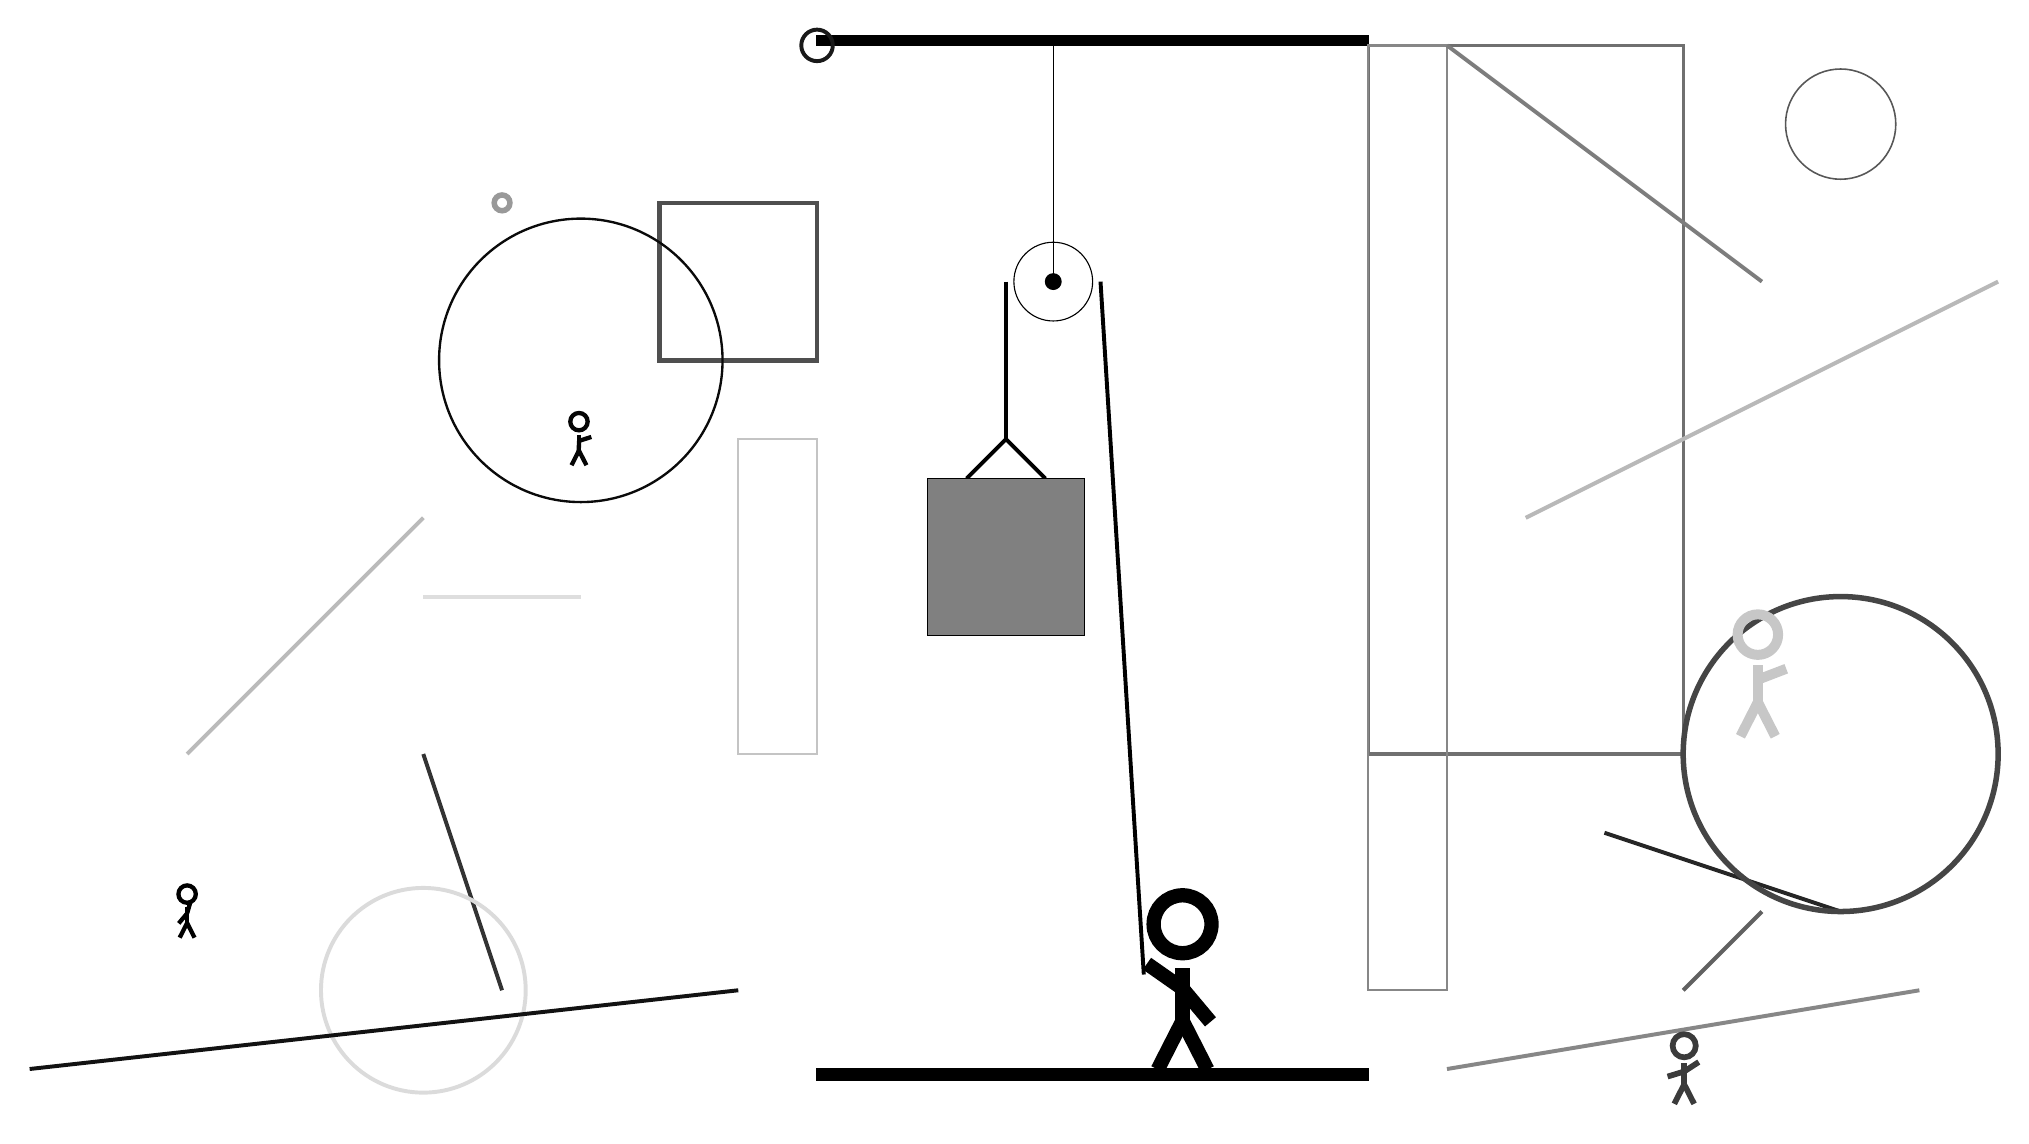
\begin{tikzpicture}
		%%%%% START %%%%%
		
		\draw[fill=black] (-2, 10) rectangle (5, 10.125);
		
		\draw (1, 7) circle (0.5);
		\draw[fill=black] (1, 7) circle (0.1);
		\draw (1, 10) -- (1, 7);
		
		\draw[line width=0.5mm] (-0.1, 4.5) -- (0.4, 5.0) -- (0.9, 4.5);
		\draw[fill=black!50] (-0.6, 4.5) rectangle (1.4, 2.5);
		
		\draw[line width=0.5mm] (0.4, 7) -- (0.4, 5.0);
		\centerarc[line width=0.5mm](1, 7)(0:180:0.6);
		\draw[line width=0.5mm](1.6, 7) -- (2.15, -1.8);
		
		\node at (2.6, -1.9) {\Strichmaxerl[10][-35][-50]};
		
		\draw[line width=0.5mm, color=black!80](-7, 1) -- (-6, -2);
		
		\draw[line width=0.4mm, color=black!56] (5, 10) rectangle (9, 1);
		\draw[line width=0.5mm, color=black!27](-7, 4) -- (-10, 1);
		\draw[line width=0.5mm, color=black!85](8, 0) -- (11, -1);
		
		\draw[line width=0.5mm, color=black!62](9, -2) -- (10, -1);
		\node[line width=0.2mm, color=black!98] at (-5, 5) {\Strichmaxerl[3][89][18]};
		\draw [line width=0.7mm, color=black!40](-6, 8) circle (0.1);
		\draw [line width=0.5mm, color=black!14](-7, -2) circle (1.3);
		\draw[line width=0.6mm, color=black!69] (-4, 8) rectangle (-2, 6);
		
		\draw[line width=0.3mm, color=black!47] (6, 10) rectangle (5, -2);
		\draw [line width=0.3mm, color=black!96](-5, 6) circle (1.8);
		
		\draw[line width=0.5mm, color=black!51](6, 10) -- (10, 7);
		\draw[line width=0.5mm, color=black!47](6, -3) -- (12, -2);
		
		\draw[line width=0.5mm, color=black!13](-5, 3) -- (-7, 3);
		\node[line width=0.6mm, color=black!77] at (9, -3) {\Strichmaxerl[4][17][33]};
		\draw [line width=0.5mm, color=black!90](-2, 10) circle (0.2);
		
		\draw[line width=0.3mm, color=black!23] (-3, 1) rectangle (-2, 5);
		
		\draw [line width=0.7mm, color=black!73](11, 1) circle (2.0);
		\node[line width=0.2mm, color=black!22] at (10, 2) {\Strichmaxerl[7][90][21]};
		\draw[line width=0.5mm, color=black!28](7, 4) -- (13, 7);
		\draw[line width=0.5mm, color=black!93](-3, -2) -- (-12, -3);
		\draw [line width=0.2mm, color=black!66](11, 9) circle (0.7);
		
		\node[line width=0.7mm, color=black!100] at (-10, -1) {\Strichmaxerl[3][50][74]};
		
		\draw[fill=black] (-2, -3) rectangle (5, -3.15);
		
		%%%%% END %%%%%
	\end{tikzpicture}
\end{document}